\section{Критическое поведение взаимодействующего блуждания без самопересечений на треугольной решётке}

Основная цель данного раздела - исследование критических свойств модели ISAW на треугольной решётке (далее, TrISAW).
Данная задача решалась ранее, в статье \cite{Privman1986}, использованием приближений наблюдаемых величин рядями Тейлора.
Полученная оценка точки фазового перехода для TrISAW выписана на таблице \ref{tab:crits}.

В данном разделе мы воспользуемся известными данными о шкалировании радиуса между краями блуждания $R^2_N$:
на основании результатов о невзаимодействующем блуждании без самопересечений \cite{Rensburg2015}, а так же о критическом поведении взаимодействующего блуждания \cite{Duplantier1987} на квадратной решётке,
найдём область конформационного перехода модели и, тем самым, уточним оценку точки фазового перехода.
 

\begin{figure}[h]
\begin{subfigure}{0.49\textwidth}
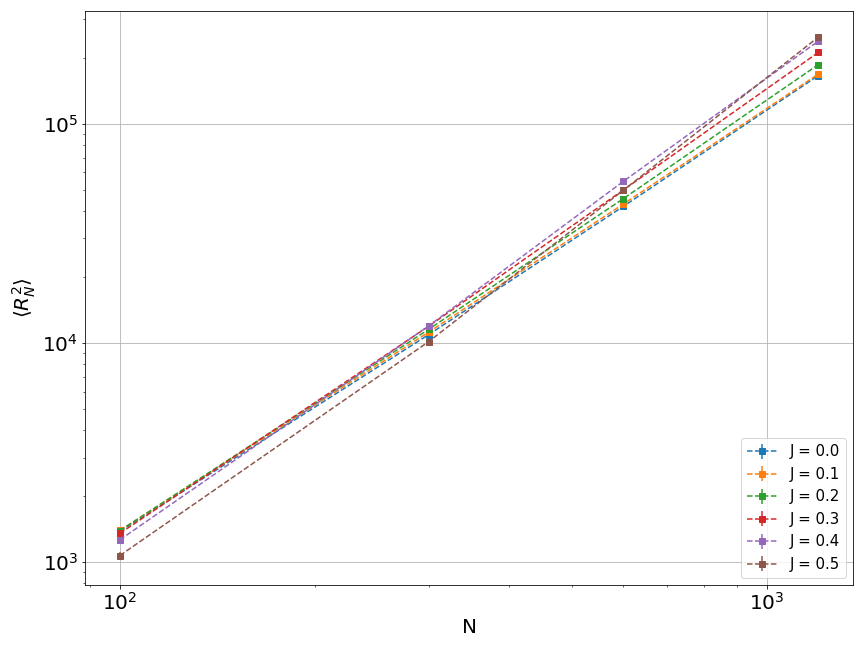
\includegraphics[width=\textwidth]{TrISAW_R2log.png}
\caption{}
\label{fig:TrISAW_R2log}
\end{subfigure}
\hfill
\begin{subfigure}{0.49\textwidth}
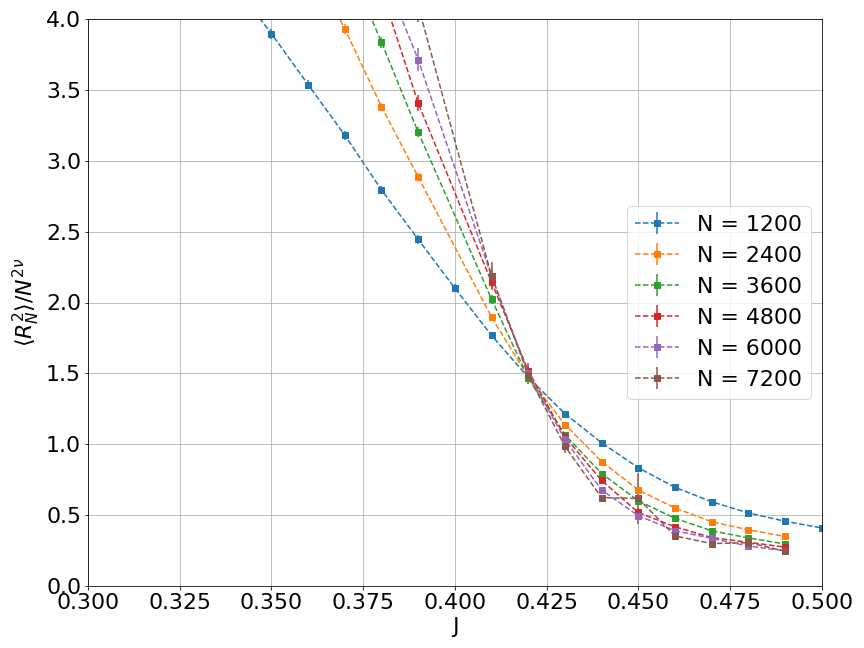
\includegraphics[width=\textwidth]{TrISAW_R2toN2v.png}
\caption{}
\label{fig:TrISAW_R2toN2v}
\end{subfigure}
\caption{Слева: Расстояние между концами блужданий длины $N$ при $J \in [0.51,0.59]$ в логарифмическом масштабе. 
Для наглядности добавлены линии $N^{2\nu}$, где $\nu = 4/7$ (красная линия) и $\nu=3/4$ (чёрная линия).
Справа: отношение расстояния между концами блуждания $R^2$ к $N^{2\nu}$, где $\nu=4/7$ при $J \in [0.52,0.58]$}
\end{figure}